% BEGIN PREAMBEL
\documentclass[9pt]{beamer}
\usepackage[british]{babel}
\usepackage{multimedia}
\usepackage{amsmath,amsfonts,amssymb}
\usepackage{upgreek}
\usepackage{pgfpages}
\usepackage[version=3]{mhchem}
\usepackage{lmodern}
\usepackage{graphicx}
\usepackage{multicol}
\usepackage{color}
\usepackage{xcolor,fontawesome}
\usepackage{wrapfig}
\usepackage{siunitx}
\usepackage{fontspec}
\usepackage{tikz}
\usepackage{textpos}
\usepackage{booktabs}
\usepackage{caption}
\usepackage{subcaption}
\usepackage{wasysym}
\usepackage{animate}
\usepackage{media9}
\usepackage{multimedia}
\newfontfamily\ubuntu{Ubuntu}
\newcommand{\as}{\\[14pt]}
\newcommand{\s}{\\[7pt]}
\newcommand{\is}{\\[2pt]}
\newcommand{\no}{\noindent}
\newcommand{\ka}{\hspace*{0.5cm}}
\newcommand{\ma}{\hspace*{1cm}}
\newcommand{\ga}{\hspace*{1.5cm}}
\newcommand{\li}{\left|}
\newcommand{\re}{\right|}
\newcommand{\const}{\text{const.}}
\newcommand{\z}{\text}
\newcommand{\terminal}[1]{\colorbox{black}{\textcolor{white}{{\fontfamily{phv}\selectfont \scriptsize{#1}}}}}
\newcommand{\plugin}[1]{\textit{\flq#1\frq}}
\newcommand{\ra}{$\rightarrow$ }
\definecolor{cadmiumgreen}{rgb}{0.0, 0.42, 0.24}
\newcommand{\itemfill}{\setlength{\itemsep}{\fill}}
\usetheme{Boadilla}
\graphicspath{ {Pics/} }
\makeatletter
\def\input@path{ {sections/} }
\makeatother
\usecolortheme{beaver}
\useoutertheme{miniframes}
\beamertemplatenavigationsymbolsempty
\makeindex
\title[Diamond Beam Tests]{Beam Tests Investigating Diamond as Detector Material}
\author[M. Reichmann]{Michael Reichmann}
\institute[\textbf{\textit{ETH}}\scalebox{.6}{\textit{Z\"{u}rich}}]{Swiss Federal Institute of Technology Zurich}
\AtBeginSection{\frame{\sectionpage}}
% END PREAMBEL

\begin{document}

% ============= TITLE PAGE =============
\usebackgroundtemplate{\tikz\node[opacity=0.2] {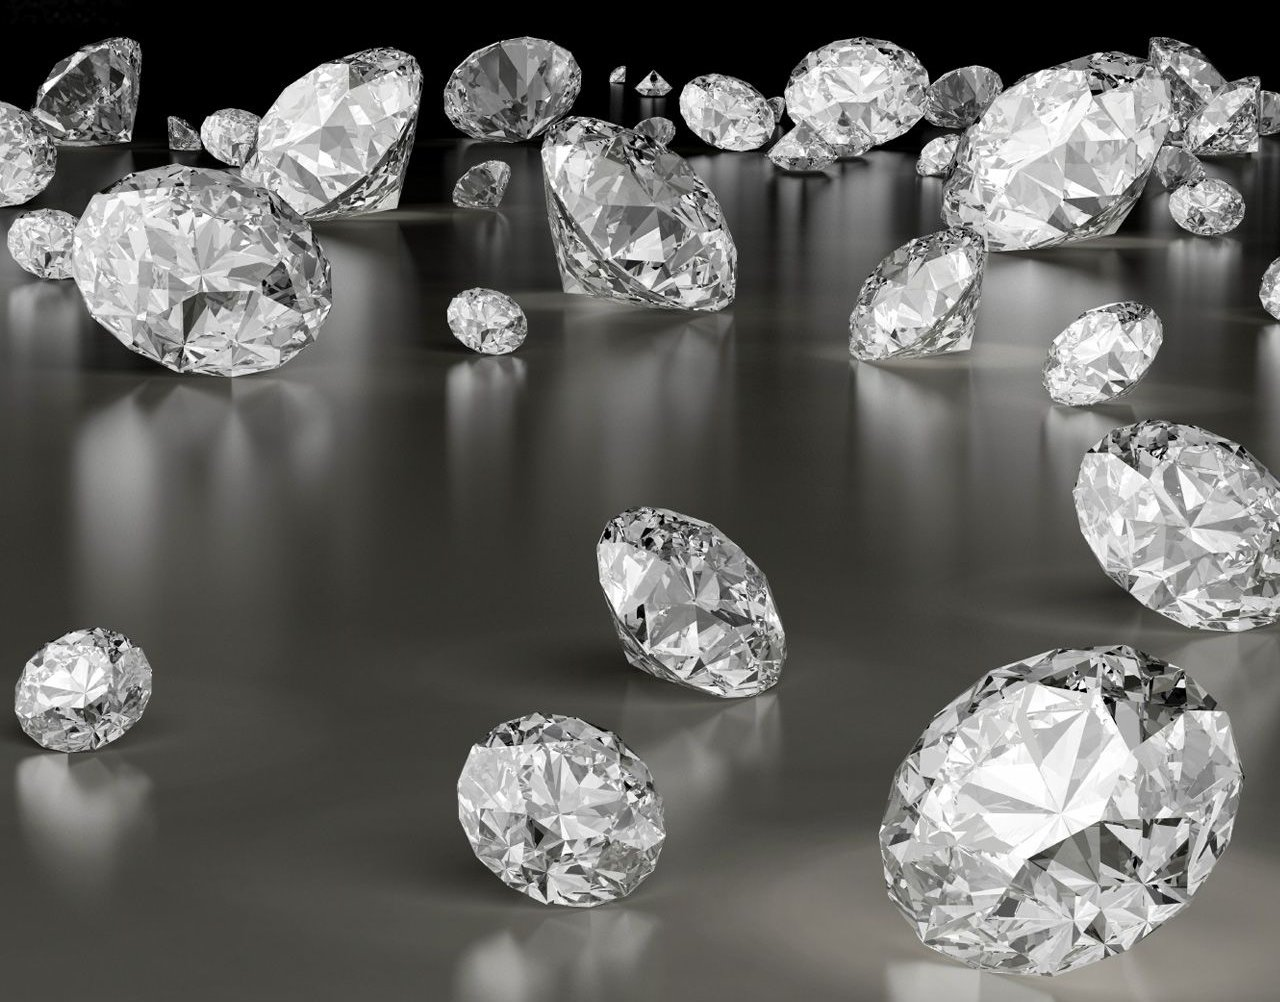
\includegraphics[height=\paperheight,width=\paperwidth]{bkg.jpg}};}
\begin{frame}
	\begin{center}
		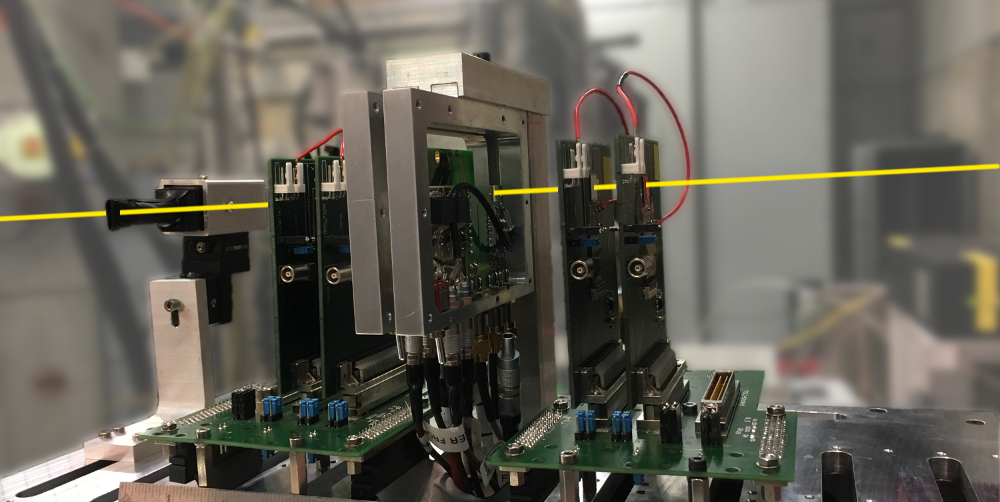
\includegraphics[width=.8\textwidth]{TitlePage}
	\end{center}
	\begin{alertblock}{
		\begin{center}
			\textbf{High Rate Beam Telescope Based on CMS Pixels}
		\end{center}}
		\vspace*{10pt}
		\begin{center}\small
		Michael Reichmann
		\end{center}\normalsize
	\end{alertblock}
\end{frame}
% END
\usebackgroundtemplate{}

% ============= TABLE OF CONTENTS ======
\begin{frame}%[allowframebreaks]
	\frametitle{Table of contents}
	\tableofcontents[hideallsubsections]   % [pausesections]
\end{frame}

% ============= TODOS =============
\section{Todo List}
\begin{frame}
	\begin{figure}
		\centering
		\animategraphics[loop, controls, width=.7\textwidth]{20}{tp}{1}{6}
	\end{figure}
\end{frame}



% ============= EFFICIENCY =============
% \section{Efficiency}
% \begin{frame}
	\frametitle{Hits in Diamond and Silicon}
	\begin{figure} 
		\begin{center}
			\begin{subfigure}{0.45\textwidth}  
				\centering 
				\includegraphics[angle=270, width=.85\textwidth]{HitsDiaSi}
			\end{subfigure}
			\begin{subfigure}{0.45\textwidth} 
				\centering 
				\includegraphics[angle=270, width=.85\textwidth]{HitPie}
			\end{subfigure} 
		\end{center}
	\end{figure}
	\begin{itemize}
		\item many cases where only Silicon or Diamond was hit (but not both)
	\end{itemize}
\end{frame}
% =============== FRAME 7 ================
\begin{frame}
	\frametitle{Trigger Phase}
	\begin{figure} 
		\begin{center}
			\begin{subfigure}{0.45\textwidth}  
				\centering 
				\includegraphics[angle=270, width=.85\textwidth]{TrigPhaseDia}
				\caption{hit in dia}
			\end{subfigure}
			\begin{subfigure}{0.45\textwidth} 
				\centering 
				\includegraphics[angle=270, width=.85\textwidth]{TrigPhaseSi}
				\caption{hit in sil}
			\end{subfigure} 
		\end{center}
	\end{figure}
	\begin{itemize}
		\item trigger phase = time with respect to the DTB clock when trigger arrives
		\item one unit = \SI{2.5}{ns}
		\item both devices connected to the same DTB \ra trigger phase always the same for both devices
	\end{itemize}
\end{frame}
% =============== FRAME 8 ================
\begin{frame}
	\frametitle{Trigger Phase}
	\begin{figure} 
		\begin{center}
			\begin{subfigure}{0.45\textwidth}  
				\centering 
				\includegraphics[angle=270, width=.85\textwidth]{TrigPhaseDiaNoSi}
				\caption{no hit in silicon}
			\end{subfigure}
			\begin{subfigure}{0.45\textwidth} 
				\centering 
				\includegraphics[angle=270, width=.85\textwidth]{TrigPhaseSiNoDia}
				\caption{no hit in diamond}
			\end{subfigure} 
		\end{center}
	\end{figure}
	\begin{itemize}
		\item trigger phase if only one device was hit
	\end{itemize}
\end{frame}
% =============== FRAME 8 ================
\begin{frame}
	\frametitle{Trigger Phase}
	\begin{figure} 
		\centering 
		\includegraphics[angle=270, width=.4\textwidth]{TrigPhaseBoth}
	\end{figure}
	\begin{itemize}
		\item both devices hit
	\end{itemize}
\end{frame}

% % ============= BACKUP ====== ======
% \section*{Backup}
% \begin{frame}
	\frametitle{Detailed Vcal Calibration}
	\begin{figure} 
		\centering 
		\includegraphics[width=\textwidth]{VcalCalibBackup}
	\end{figure}
\end{frame}

% DOCUMENT END
\end{document}

